\documentclass{article}
\usepackage[margin=1.5cm,bottom=2cm]{geometry}
\usepackage{fancyhdr}
\usepackage{graphicx}
\pagestyle{fancy}
\usepackage{enumitem,amssymb}
\newlist{todolist}{itemize}{2}
\setlist[todolist]{label=$\square$}

\begin{document}
\fancyhead[L]{ 
\includegraphics[width=2cm]{au_logo.png} }
\fancyhead[R]{PHYS 2250: General Physics II}
\fancyfoot[C]{\thepage}
\vspace*{0cm}
\begin{center}
	{\LARGE \textbf{Quiz 2}}
	%\vspace{0.25cm}
	%{\Large Due: Friday, September 11}
\end{center}
You may or may not make use of the following:
\vspace{.5cm}

\renewcommand{\arraystretch}{2}
\begin{tabular}{ccc}
$\epsilon_0=8.85\times10^{-12}\ Nm^2C^{-2}$ & $k=\frac{1}{4\pi\epsilon_0}=9\times10^9\ C^2N^{-1}m^{-2}$\\
$|\vec{E}_\mathrm{dipole,on-axis}| \approx \frac{1}{4\pi\epsilon_0}\frac{2p}{r^3}$ & $|\vec{E}_\mathrm{dipole,perp}| \approx \frac{1}{4\pi\epsilon_0}\frac{p}{r^3}$
\end{tabular}
%Complete the following problems from your textbook at the end of Chapter 13.
\begin{enumerate}
\item Which of the following are true? Check ALL that apply.
	\begin{todolist}
		\item If the net electric field at a particular location inside a piece of metal is zero, the metal is not in equilibrium
		\item The net electric field inside a block of metal is zero under all circumstances
		\item The net electric field at any location inside a block of copper is zero if the copper block is in equilibrium
		\item The electric field from an external charge cannot penetrate to the center of a block of iron
		\item In equilibrium, there is a net flow of mobile charges inside a conductor
	\end{todolist}

\begin{figure}[ht!]
	\centering
	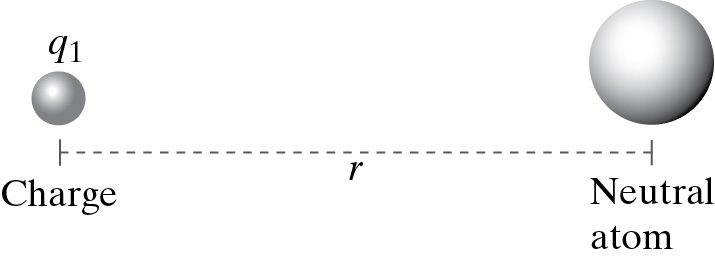
\includegraphics[width=0.5\textwidth]{..//lectures/figures/Ch14jpegs/fig1479.jpg}
\end{figure}

\item Consider the diagram above, where $q_1$ is a charged particle and the atom is neutral.

\begin{enumerate}
	\item If $q_1$ is negative in the above diagram, which of the configurations below (1-10) best describes the charge distribution in the neutral atom in this situation? If other, please specify.


\begin{figure}[ht!]
	\centering
	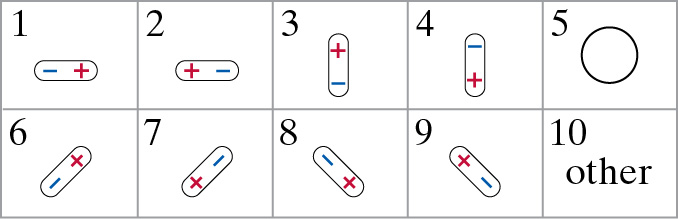
\includegraphics[width=0.5\textwidth]{..//lectures/figures/Ch14jpegs/fig1480.jpg}
\end{figure}

\item Which arrow below best describes the direction of the electric field at the location of $q_1$ due to the polarized neutral atom?

\begin{figure}[ht!]
	\centering
	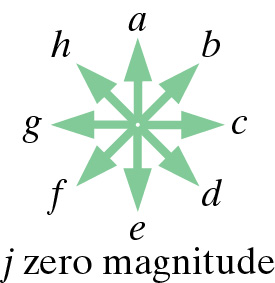
\includegraphics[width=0.2\textwidth]{..//lectures/figures/Ch14jpegs/fig1481.jpg}
\end{figure}
\item Which of the arrows best describes the direction of the force on the charged particle, due to the polarized atom?
\end{enumerate}
\end{enumerate}

\end{document}